\chapter{Introduzione}

Il tirocinio è stato svolto all'interno del progetto \textbf{SeismoCloud}.\\
Di seguito viene innanzitutto introdotto il progetto stesso, mostrandone la struttura, lo scopo ed una visione ad alto livello del funzionamento delle sue componenti. Si trattano poi l'inserimento all'interno del team di sviluppo e gli strumenti utilizzati per tutta la durata del tirocinio.


\section{SeismoCloud, Earthquake Early Warning system}

\begin{wrapfigure}{r}{0.25\textwidth}
    \centering
    
\includegraphics[scale=0.15]{images/seismologo.png}
    \caption{Logo di SeismoCloud}
    \label{fig:seismologo}
\end{wrapfigure}

SeismoCloud \cite{seismocloud} è un progetto nato nel grazie al connubio dell'Università degli Studi di Roma “La Sapienza” e l’Istituto Nazionale di Geofisica e Vulcanologia (INGV). L'idea alla base del progetto è la rilevazione in tempo reale di scosse sismiche mediante una rete di sensori a basso costo e la segnalazione di un imminente terremoto alla popolazione della zona colpita tramite un'applicazione per dispositivi mobile. Il nome di quest'ultima ricalca il nome del progetto: \textit{SeismoCloud} (il logo è riportato nella Figura \ref{fig:seismologo}). Un sistema con queste finalità prende il nome di \textit{Earthquake Early Warning} (EEW).\\
\\
I dispositivi utilizzati per rilevare le scosse sismiche (da qui in avanti nominati \textit{Sismometri}) hanno un grande vantaggio che ne permette la rapida e semplice diffusione: il prezzo contenuto. Questa caratteristica consente alla rete di Sismometri di espandersi per sopperire all'unico svantaggio che si contrappone al modico prezzo: la precisione. Difatti, le rilevazioni di un singolo sismometro sono altamente imprecise, rendendo comuni vibrazioni (provocate, ad esempio, dal passaggio di una persona sulla stessa superficie su cui è posto il sismometro) un potenziale allarme. La costituzione di una fitta rete di Sismometri è essenziale per rendere il sistema completamente operativo ed affidabile nell'invio delle segnalazioni agli utenti dell'applicazione, motivo per cui, attualmente, la funzione di notifica preventiva non è ancora attiva.

\paragraph{I Sismometri}
I Sismometri sono i più validi alleati per la rilevazione delle scosse sismiche. La componente responsabile della misurazione delle vibrazioni prende il nome di \textbf{accelerometro}. Esso ne misura il valore basandosi sulla variazione di accelerazione che le scosse provocano su di ad esso.\\
L'accelerometro in sé, tuttavia, non ha una vera utilità se non viene collegato ad un dispositivo che lo gestisce e che invia i dati raccolti tramite Internet a SeismoCloud. Le alternative spaziano tra l'utilizzo di Raspberry Pi \cite{rpi} e di NodeMCU \cite{nodemcu}, dispositivi tipici dell'IoT, oltre che i dispositivi mobile stessi, dotati di un accelerometro. Sul sito web ufficiale di SeismoCloud \cite{seismocloud} è possibile trovare precise istruzioni su come creare il proprio sismometro con le componenti di cui sopra; inoltre, il codice per la loro configurazione è Open Source, disponibile sul profilo GitHub del progetto \cite{seismogit}. \\
La Figura \ref{fig:seismometers} mostra i Sismometri attivi sul territorio nazionale.

\begin{figure}[h!]
    \centering
    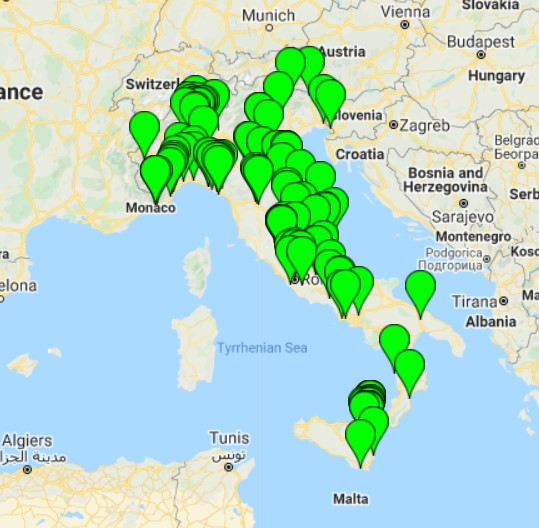
\includegraphics[width=\textwidth]{images/seismometersjpg.jpg}
    \caption{Sismometri attivi a livello nazionale}
    \label{fig:seismometers}
\end{figure}

\paragraph{Come si identifica un terremoto}
Si è discusso di quali sono gli elementi principali per la rilevazione delle scosse. Essi non sono però responsabili in maniera diretta della decisione da prendere sulla natura della scossa: questa decisione viene delegata al server che riceve i dati dei Sismometri. Grazie a degli algoritmi dedicati al processing delle informazioni sulle scosse in input, il server calcola se la vibrazione in cui sono incorsi i Sismometri è riconducibile ad una scossa sismica, e, a quel punto, aziona il meccanismo di Early Warning. 

\paragraph{La segnalazione}
Il sistema di EEW ha la capacità di salvare secondi preziosissimi agli utenti in caso di scossa sismica: si parla, difatti, di un avvertimento dai \textbf{2} ai \textbf{20} \textbf{secondi} prima dell'avvenimento del terremoto nel luogo in cui ci si trova, tempo utile non a fuggire ma a cercare riparo ed avere salva la vita.
A livello tecnico, la segnalazione di una scossa avviene tramite l'applicazione, che scatena la vibrazione tipica del ricevimento di una notifica sul dispositivo mobile. Vista l'importanza che questa notifica ha in caso di effettivo terremoto , la vibrazione può essere personalizzabile; inoltre, nei dispositivi Android, è possibile consentire all'applicazione di far vibrare il telefono anche se in modalità "silenziosa".

\paragraph{L'applicazione}

L'applicazione SeismoCloud, mostrata nella Figura \ref{fig:application}, rappresenta il punto di accesso a tutte le funzionalità offerte, come il monitoraggio dei propri Sismometri (Bottone \textit{Seismo} nella navigation bar), la visualizzazione del proprio profilo e delle impostazioni dell'applicazione (bottone \textit{Settings}), dei terremoti o delle scosse rilevate recentemente (bottone \textit{Quakes}, la schermata su cui ci si trova nell'immagine mostrata), dei gruppi di cui si è parte (bottone \textit{Groups}) e dei sensori presenti su una mappa (bottone \textit{Map}). 
Una delle funzioni fondamentali è raggiungibile cliccando su uno dei terremoti presenti nella lista (riportata in Figura \ref{fig:applicationsurvey}): oltre a presentare dei dati fondamentali relativi al terremoto (come l'istante di rilevamento, la sua posizione tramite visualizzazione sulla mappa, la distanza dalla posizione attuale del dispositivo attuale, la magnitudo del terremoto ed altre informazioni), l'applicazione permette agli utenti di rispondere ad un sondaggio in cui si chiedono dettagli su dove ci si trovasse, su cosa si facesse e su cosa si è percepito al momento del terremoto. Altre caratteristiche importanti sono accessibili tramite il bottone \textit{Settings}: è difatti possibile personalizzare la ricezione di una notifica in caso di Early Warning anche se in modalità silenziosa, attivare o disattivare la rilevazione tramite il sensore del dispositivo mobile e stabilire il consumo energetico massimo che l'applicazione attiva comporta (per approfondire quest'ultimo punto, consultare il lavoro di Enrico Bassetti \cite{enricobassetti}).

\begin{figure}[h]

\begin{subfigure}{0.5\textwidth}
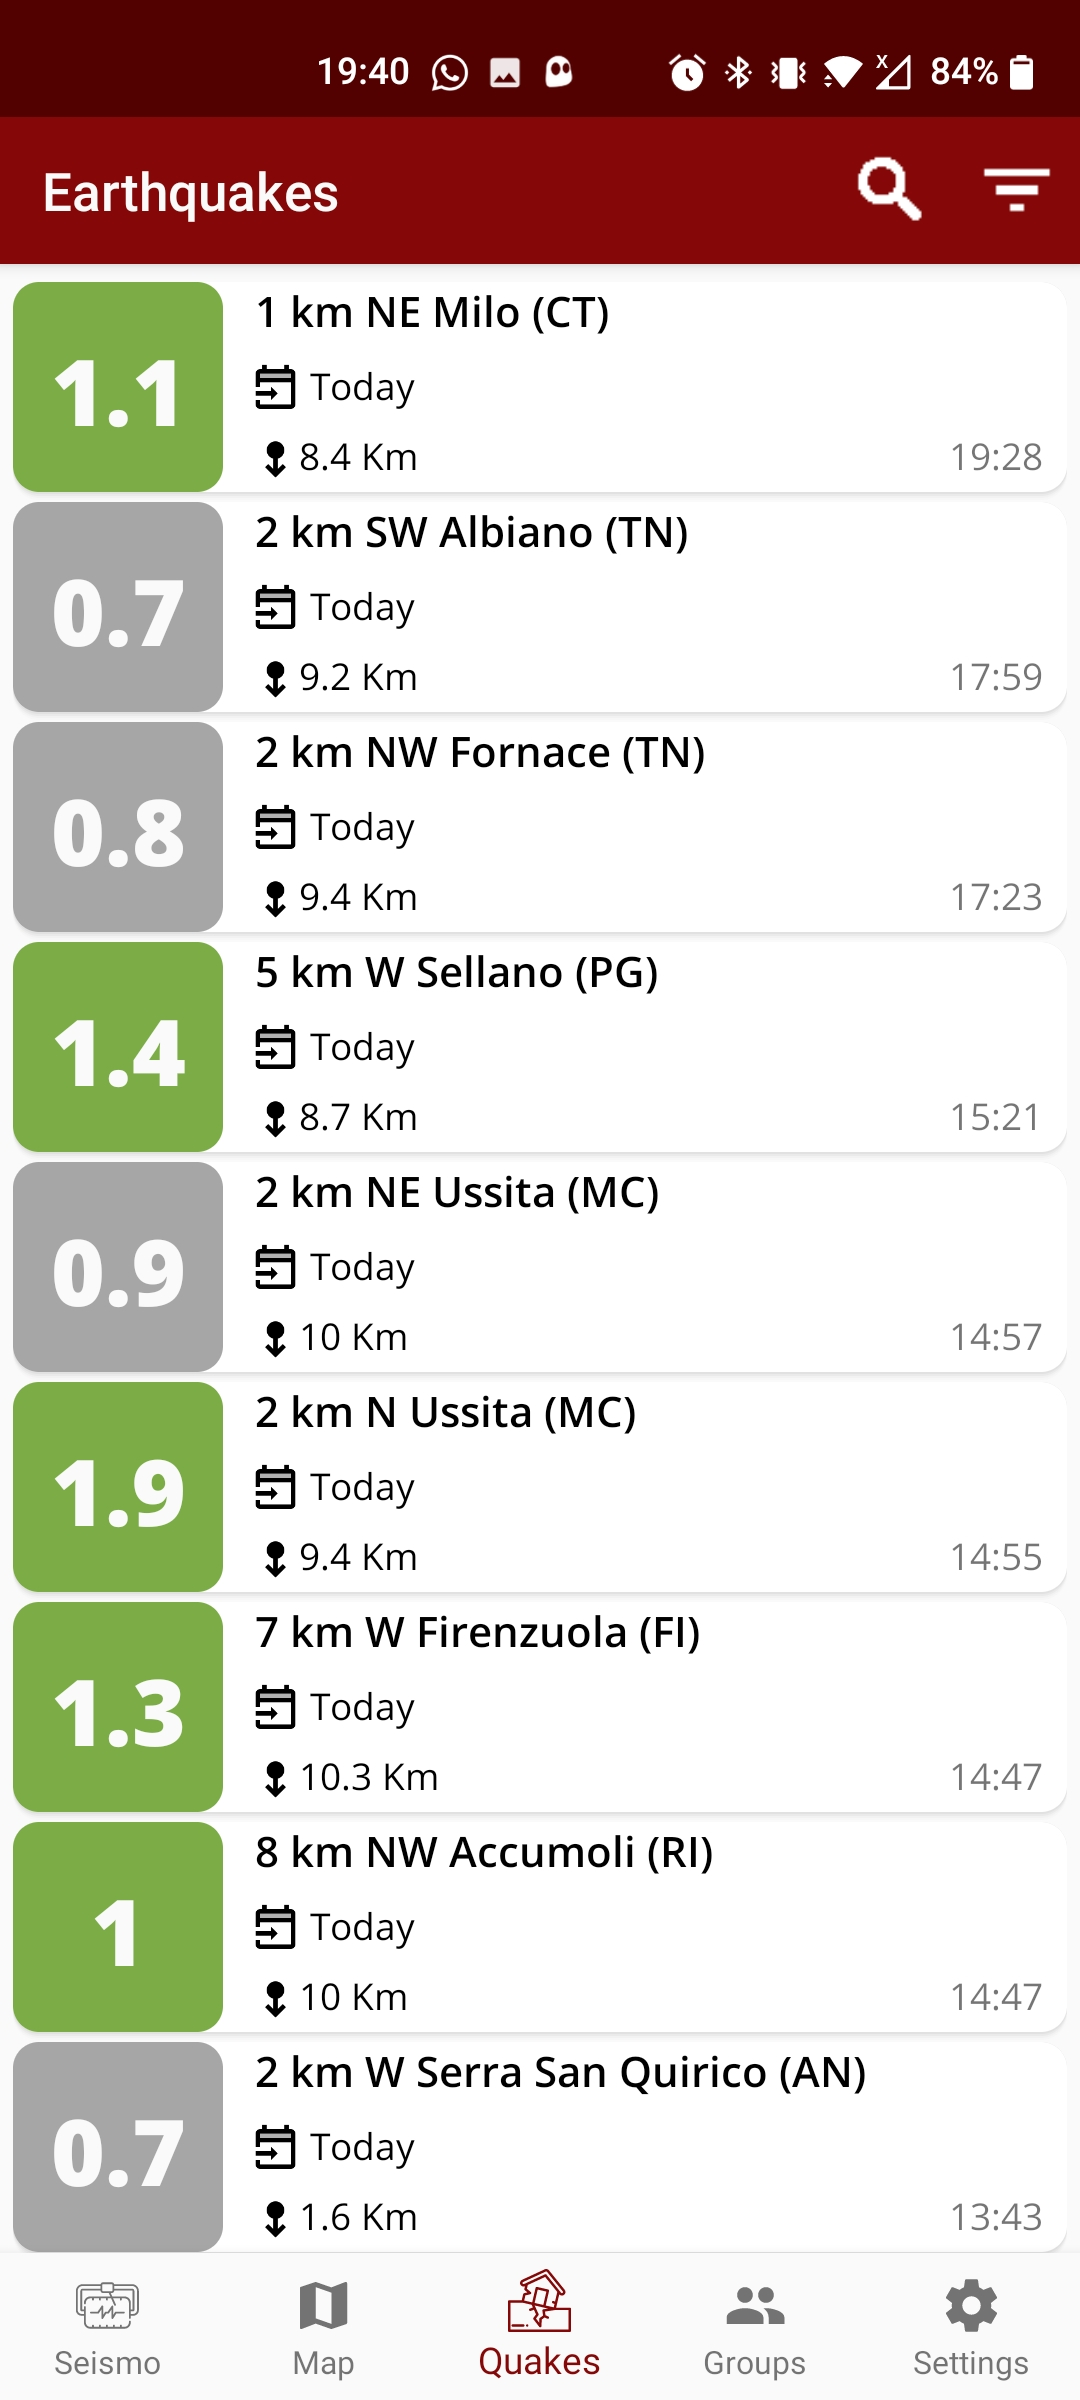
\includegraphics[width=0.9\linewidth]{images/application.png} 
\caption{Schermata dei terremoti}
\label{fig:application}
\end{subfigure}
\begin{subfigure}{0.5\textwidth}
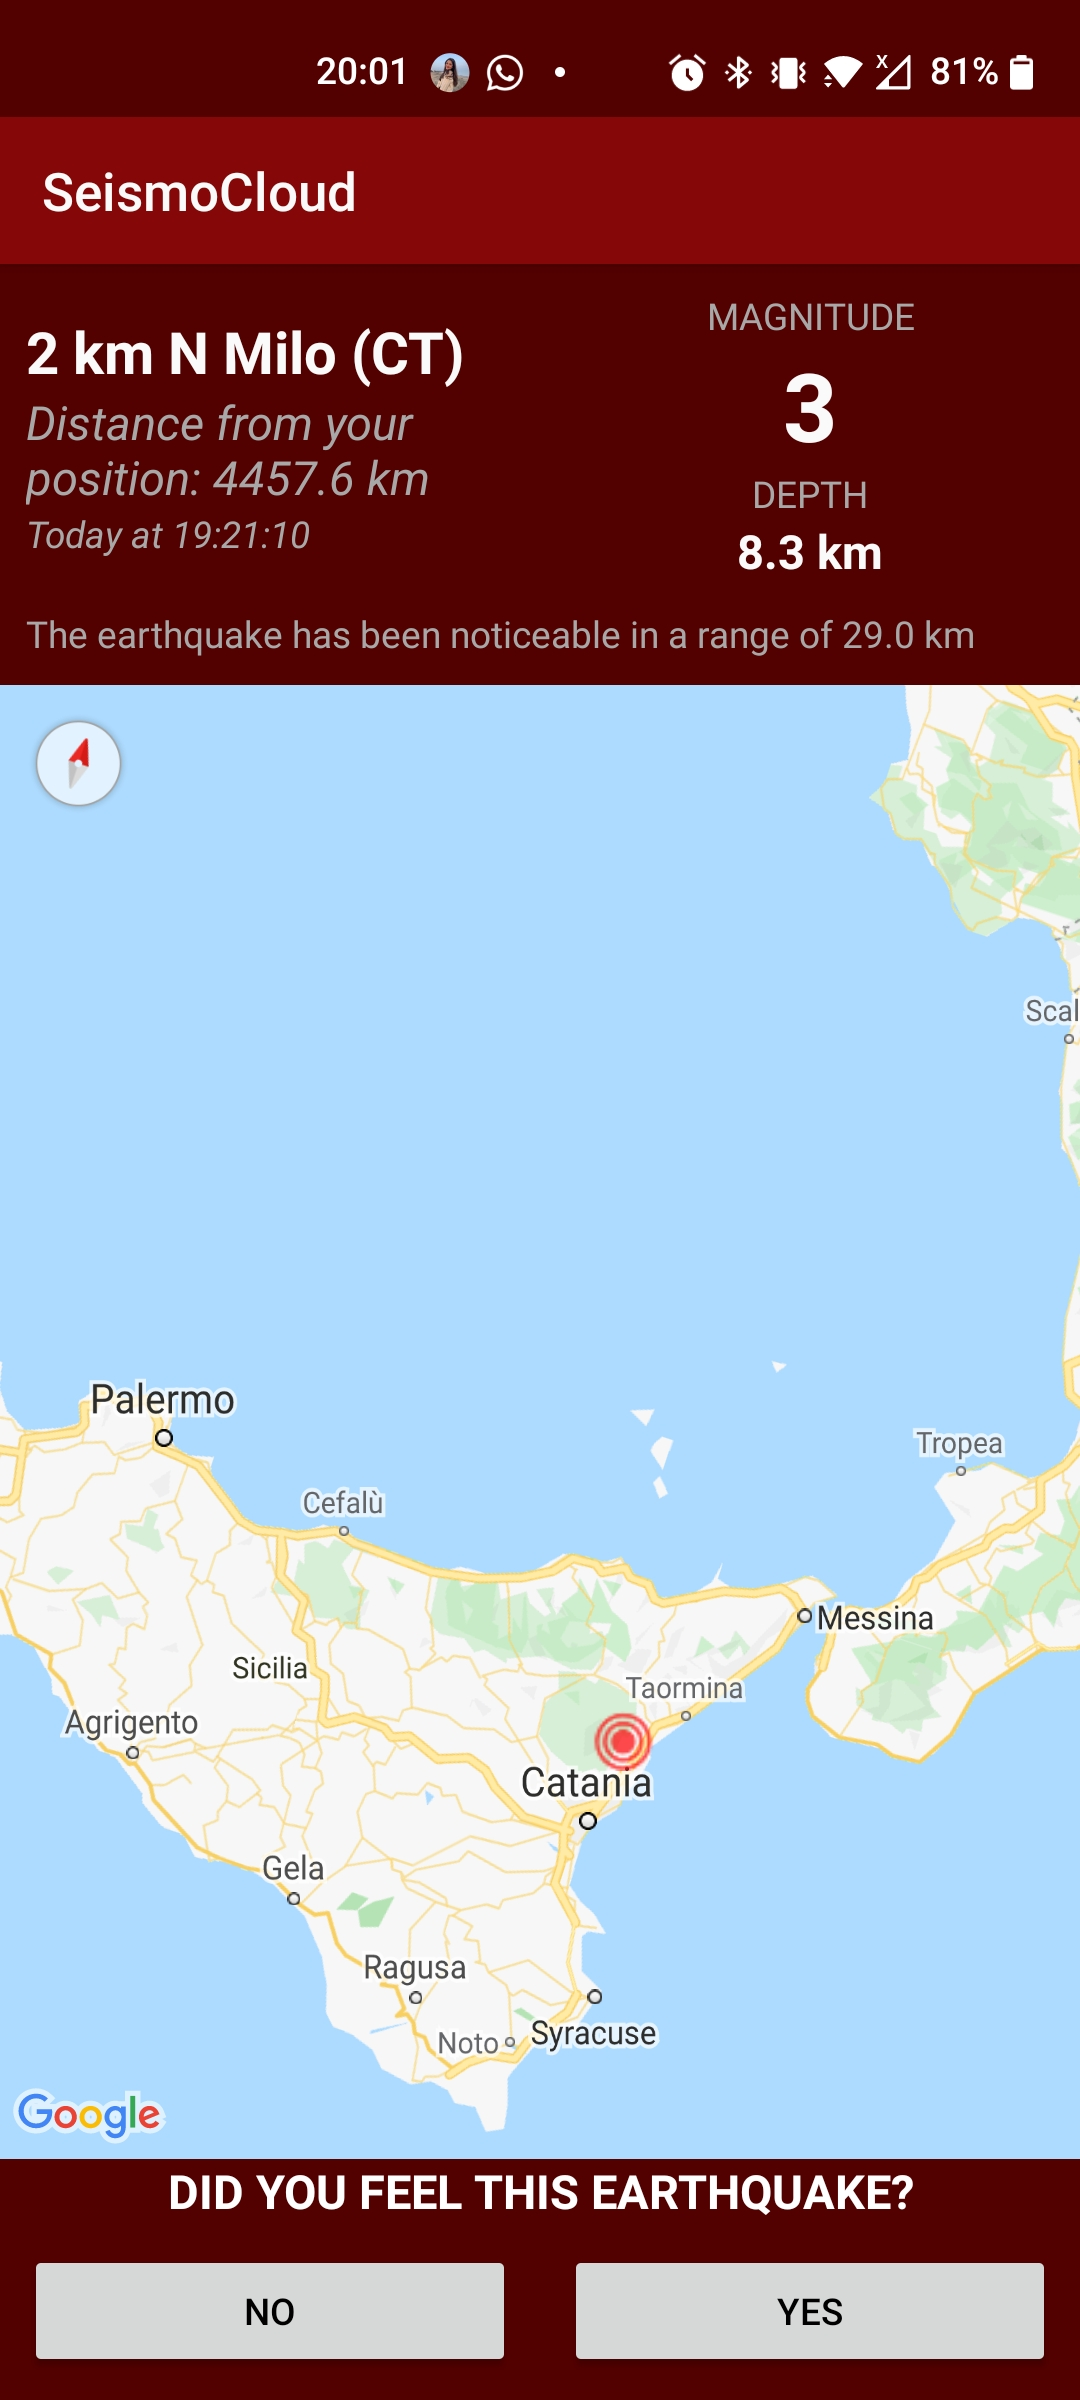
\includegraphics[width=0.9\linewidth]{images/applicationsurvey.png}
\caption{Schermata relativa ad un terremoto}
\label{fig:applicationsurvey}
\end{subfigure}

\caption{Schermate dell'applicazione SeismoCloud}
\label{fig:schermate}
\end{figure}

\section{Organizzazione del workflow}

Parte fondamentale del tirocinio è stata partecipare attivamente al progetto assieme ad altri tirocinanti e colleghi, con riunioni settimanali programmate per discutere il lavoro svolto nel time frame settimanale precedente, per chiarire dubbi su problemi incontrati e per confrontarsi. Un aspetto cruciale che ha permesso la cooperazione fin dal primo istante è stato utilizzare lo strumento di Version Control \textbf{Git} \cite{git}. Grazie ad esso, è possibile utilizzare uno speciale meccanismo di "checkpoint", i \textit{Commit}, che permettono il salvataggio del lavoro svolto sulla repository del progetto; l'utilità straordinaria è la possibilità di tornare ad uno stato precedente del progetto ed effettuare cambiamenti su versioni diverse del codice, non necessariamente secondo un ordine cronologico di cambiamenti. Ciò permette di ritornare sui propri passi nel caso in cui il codice modificato rispetto ad un \textit{Commit} precedente non permetta al sistema di funzionare correttamente. Se si ha l'urgenza di riportare il sistema ad una versione stabile, questa funzionalità appare ancora più funzionale.\\
Un secondo aspetto importante vede protagonisti i \textit{Branch}. Un \textit{Branch} rappresenta la linea temporale demarcata dai \textit{Commit} effettuati sul \textit{Branch} stesso. Possono essere creati moltissimi \textit{Branch}, ed è buona pratica seguire questa condotta: è sempre bene creare un \textit{Branch} per ogni nuova funzionalità che si sta implementando, per ogni \textit{hotfix} necessario a ripristinare il corretto funzionamento di una componente e per molti altri scenari.\\
Durante tutto lo svolgimento del tirocinio è stato necessario lavorare su uno o più \textit{Branch}, sia per non andare ad intaccare l'applicazione sottostante con dei cambiamenti e delle problematiche inevitabilmente introdotte nel corso dell'implementazione, sia per non entrare in conflitto con altri membri del team, ad esempio nella scrittura concorrente sullo stesso file.\\
\textit{Git} conta innumerevoli funzioni e comportamenti per favorire un ambiente di sviluppo quanto più organizzato e gestito possibile; si rimanda alla documentazione ufficiale dei comandi per una versione approfondita \cite{git}. 